%%%%%%%%%%%%%%%%%%%%%%%%%%%%%%%%%%%%%%%%%%%%%%%%%%%%%%%%%%%%%%%%%%%%%%%%%%
%%%%%                         CHAPITRE 2                            %%%%%%
%%%%%%%%%%%%%%%%%%%%%%%%%%%%%%%%%%%%%%%%%%%%%%%%%%%%%%%%%%%%%%%%%%%%%%%%%%

\lhead[\fancyplain{}{\leftmark}]%Pour les pages paires \bfseries
      {\fancyplain{}{}} %Pour les pages impaires
\chead[\fancyplain{}{}]%
      {\fancyplain{}{}}
\rhead[\fancyplain{}{}]%Pour les pages paires 
      {\fancyplain{}{\rightmark}}%Pour les pages impaires \bfseries
\lfoot[\fancyplain{}{}]%
      {\fancyplain{}{}}
\cfoot[\fancyplain{}{\thepage}]%\bfseries
      {\fancyplain{}{\thepage}} %\bfseries
\rfoot[\fancyplain{}{}]%
     {\fancyplain{}{\scriptsize}}


%%%%%%%%%%%%%%%%%%%%%%%%%%%%%%%%%%%%%%%%%%%%%%%%%%%%%%%%%%%%%%%%%%%%%%%%%%
%%%%%                      Start part here                          %%%%%%
%%%%%%%%%%%%%%%%%%%%%%%%%%%%%%%%%%%%%%%%%%%%%%%%%%%%%%%%%%%%%%%%%%%%%%%%%%
\renewcommand\chapterheadstartvskip{\vspace*{-2\baselineskip}}
\chapter{Simulations numériques directes}
\label{ch/DNS}

%==============================================================================	Résumé du chapitre

\begin{center}
\rule{0.8\linewidth}{.5pt}
\begin{minipage}{0.8\linewidth}
\smallskip

\textit{L'ensemble des outils numériques utilisés pendant la thèse sont introduits dans ce chapitre. Le code SND (Simulation Numérique Directe) MULTIFAST est présenté en détails dans une première section. En second temps, les implémentations additionnelles faites durant la thèse sont explicitées. Enfin, dans une troisième section, MULTIFAST est validé en reproduisant un cas académique. Quelques résultats significatifs d'un écoulement pleinement turbulent en canal sont également présentés en guise de validation.}

%\smallskip
\end{minipage}
\smallskip
\rule{0.8\linewidth}{.5pt}
\end{center}

\clearpage
\setbeforeminitoc
$~$
\vfill
\minitoc
\vfill
\newpage
\resetafterminitoc
%%%%%%%%%%%%%%%%%%%%%%%%%%%%%%%%%%%%%%%%%%%%%%%%%%%%%%%%%%%%%%

Historiquement, les plus grandes avancées dans la compréhension et la modélisation de la mécanique des fluides ont été réalisées de manière expérimentale. Cependant, les expériences peuvent être difficiles à mettre en place ou à reproduire, elles sont sensibles à divers paramètres et coûteuses d'un point de vue matériel. Davantage d'études sont donc réalisées dans le domaine de la mécanique des fluides numérique (CFD). Cependant, bien que les équations de Navier-Stokes soient connues depuis longtemps, l'existence et l'unicité d'une solution aux équations n'ont pas encore été prouvées, et cela constitue même un des problèmes du millénaire\footnote{\url{https://www.claymath.org/millennium-problems}}.

\begin{figure}[!hbtp]
    \centering
    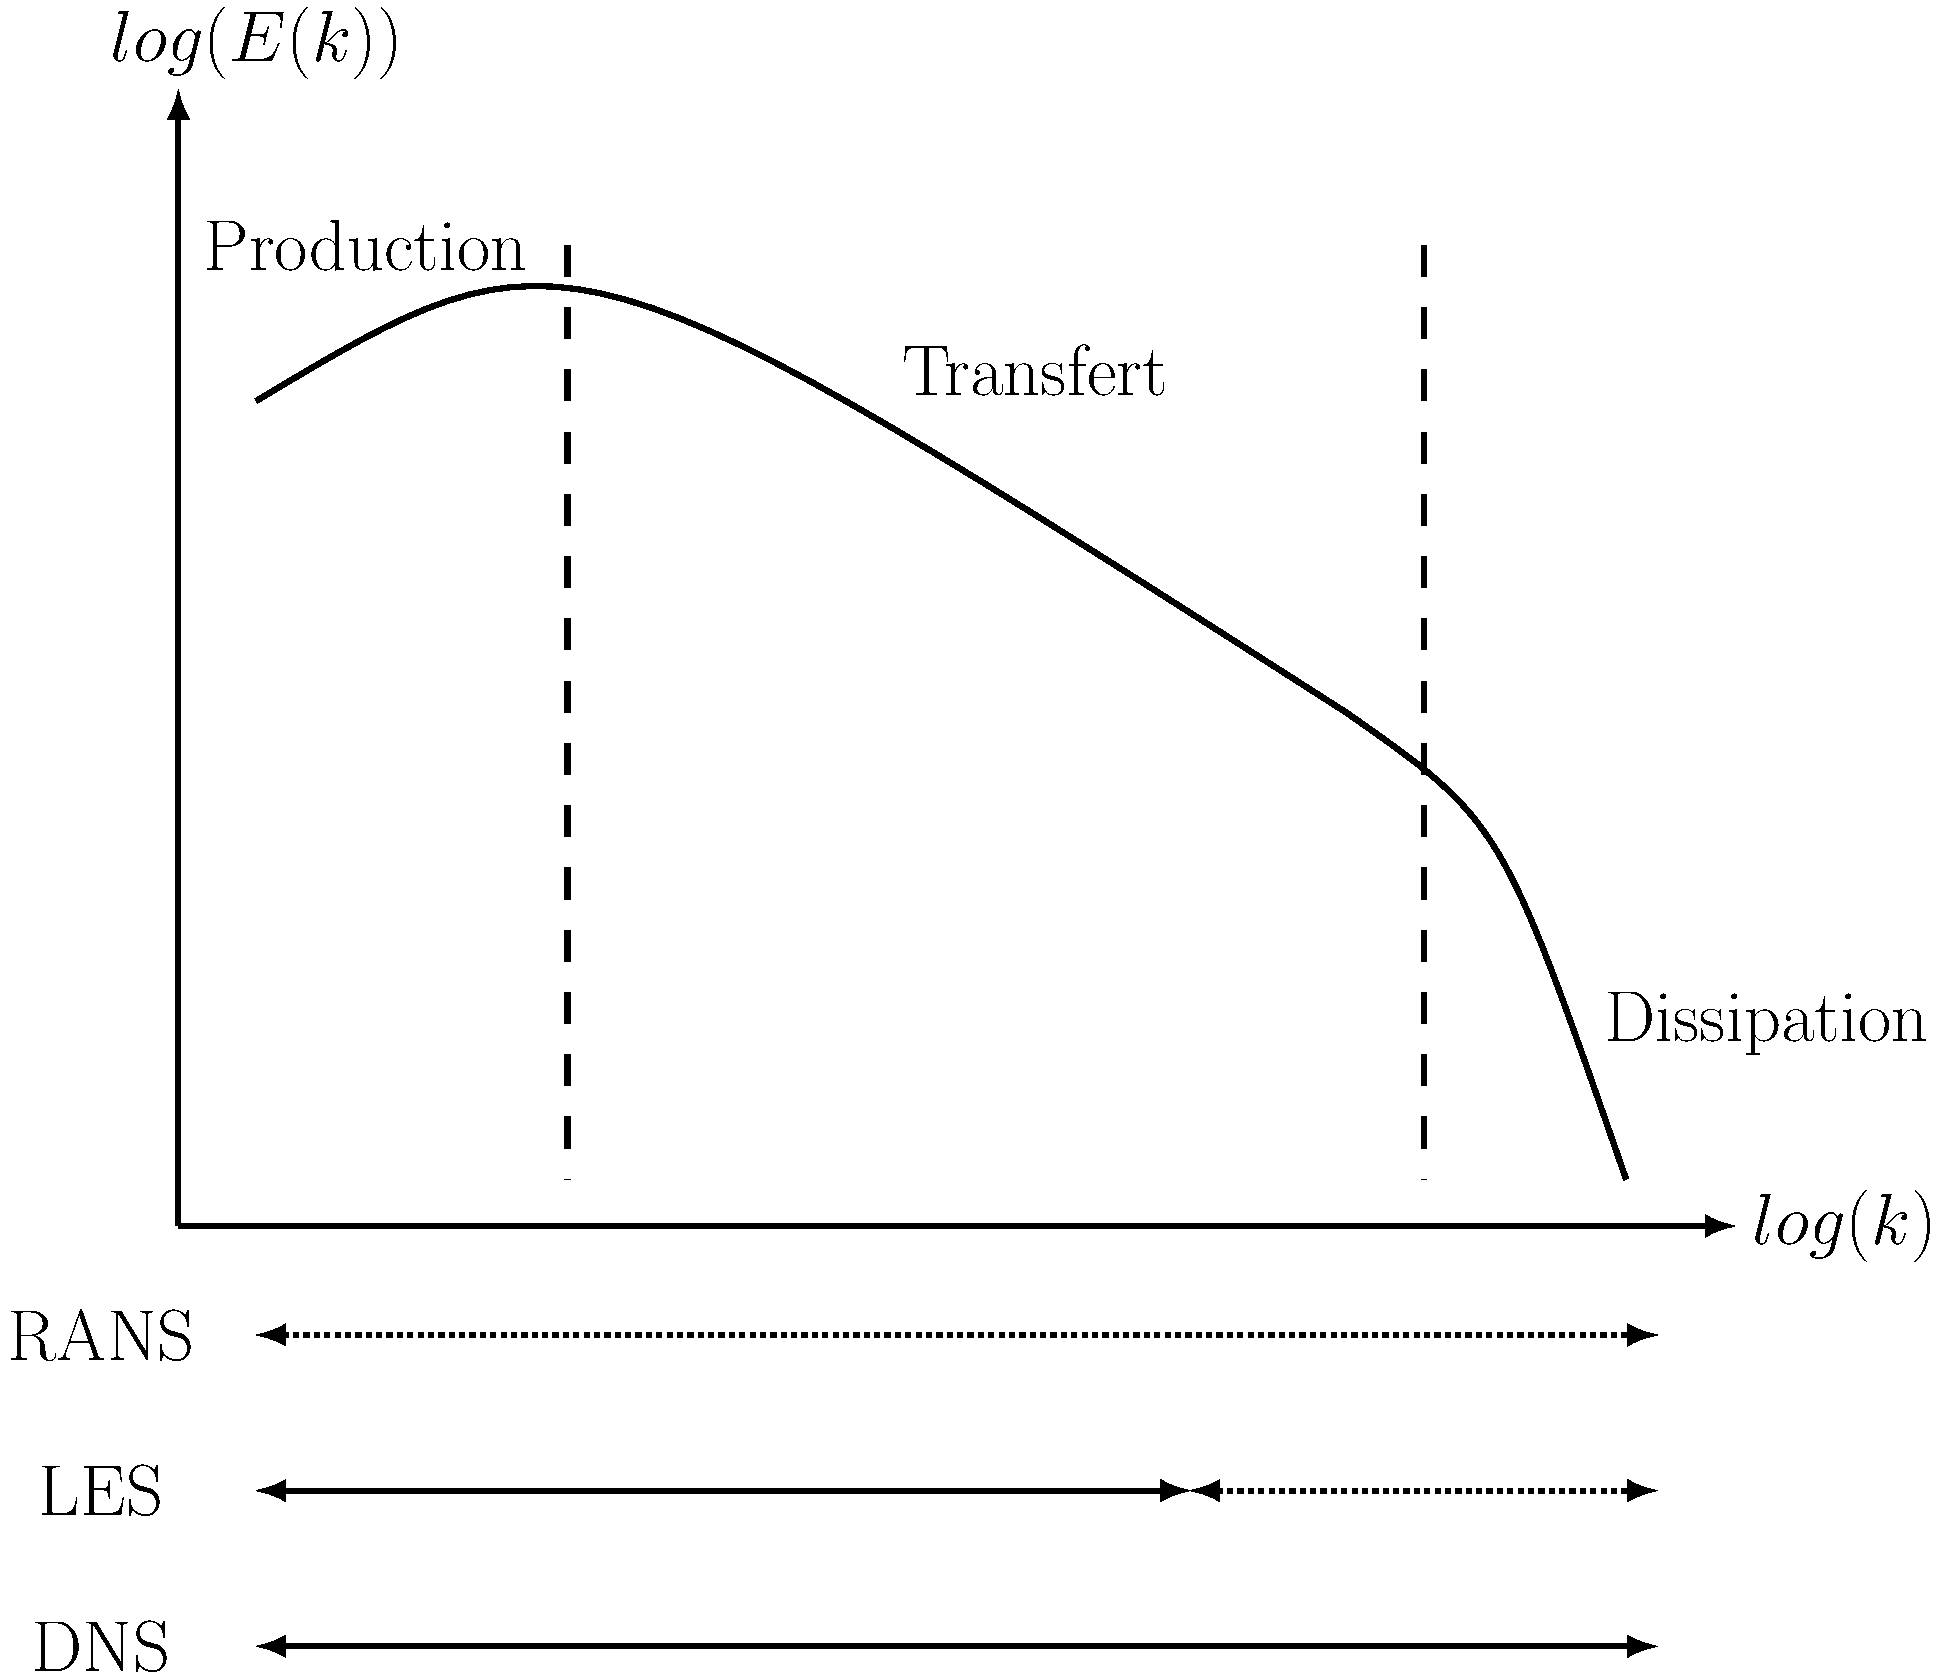
\includegraphics[width=0.7\linewidth]{Chap2/Pictures/Energy_cascade.pdf}
    \caption{Schéma illustrant la production, le transfert et la dissipation dans le spectre énergétique de la turbulence (\cite{kolmogorov1941}). Correspondance avec les différentes méthodes de simulations numériques. Les flèches en traits continus représentent les échelles de turbulence résolues, et les flèches en pointillés les échelles de turbulence modélisées.}
    \label{fig/Energy_cascade_schema}
\end{figure}

La turbulence est un état particulier d'un écoulement. Elle se caractérise par la formation, la régénération et la coexistence de structures tourbillonnaires de plusieurs tailles. Chaque structure tourbillonnaire transporte sa propre énergie qu'elle transmet à une structure tourbillonnaire de plus petite taille par diffusion turbulente, jusqu'à atteindre une taille minimale appelée \textit{échelle de Kolmogorov} (\cite{kolmogorov1941}). L'énergie transportée par les structures tourbillonnaires se dissipe par frottement dû à la viscosité du fluide pour les plus petites tailles. Il faut garder en mémoire que la méthode numérique employée doit être capable de simuler et/ou capturer tous les phénomènes et tous les tourbillons lorsque l'on veut résoudre numériquement les équations de Navier-Stokes. Plusieurs méthodes ont été envisagées, chacune ayant son propre coût numérique et sa propre précision. Les 3 principales méthodes sont :

\begin{itemize}

	\item \textbf{RANS} pour \textit{Reynolds Averaged Navier-Stokes} qui se base sur la résolution des équations de Navier-Stokes moyennées en temps ou en espace. Elle nécessite un modèle de fermeture pour les équations dont les principaux sont le $k-\epsilon$, $k-\omega$ et $k-\omega~SST$. Il faut comprendre que la méthode RANS permet de résoudre l'écoulement moyen. De plus, le modèle de fermeture peut différer suivant le type d'écoulement à résoudre. À titre d'exemple, les simulations numériques effectuées en Formule 1 sont basées sur le modèle $k-\omega~SST$.

	\item \textbf{LES} pour \textit{Large-Eddy Simulation} qui résout les grandes échelles de turbulence et modélise les plus petites échelles (\cite{Sagaut2005}). L'idée est de filtrer les plus petites échelles de la turbulence et de les modéliser. C'est une méthode qui propose un compromis entre la méthode RANS et la méthode SND. 

	\item \textbf{SND} pour \textit{Simulation Numérique Directe} résout intégralement les équations de Navier-Stokes sans aucune modélisation.
\end{itemize}

La différence majeure entre les trois méthodes réside dans ce qui est résolu et/ou modélisé. En effet, une partie (voire la totalité) des échelles est modélisée pour les simulations RANS et LES. Cela a pour conséquence qu'un maillage moyen ou grossier peut être utilisé avec de telles simulations. En revanche, le maillage utilisé doit être aussi fin que l'échelle de Kolmogorov pour une simulation SND comme toutes les échelles de la turbulence sont résolues. Bien qu'une simulation SND résolve directement les équations de Navier-Stokes, il faut davantage de ressources numériques pour mener à bien un calcul en des temps raisonnables. Une $4^{\grave{e}me}$ méthode a récemment vu le jour : la méthode Lattice-Boltzmann (LBM). Elle est basée sur une approche lagrangienne et statistique de l'écoulement. Ce ne sont pas les équations de Navier-Stokes qui sont résolues, mais l'équation de Boltzmann qui simule les collisions et la propagation des particules dans l'espace. Le lecteur intéressé peut se référer à \cite{chen1998}, \cite{mohamad2011} et \cite{Teschner_Lecture}.\\

Des simulations SND ont été choisies dans le cadre de la thèse, car les écoulements étudiés sont soit des écoulements de transition, soit des écoulements dans des canaux rugueux. La nature de l'écoulement va être modifiée au cours de la simulation dans les deux cas. Aucune approximation ni aucun modèle ne peuvent être tolérés et il faut capturer chaque échelle de la turbulence. Le rapport entre les plus grandes échelles et les plus petites échelles de la turbulence augmente avec le nombre de Reynolds ($\sim Re^{3/4}$) comme expliqué par \cite{pope2000}. La mémoire nécessaire pour le calcul est proportionnelle à $Re^{3}$ et le temps de simulation à $Re^{4}$ pour des écoulements dans des canaux. Bien que la puissance de calcul ait doublé chaque année depuis les années 1970, une simulation SND à très haut nombre de Reynolds $Re$ n'est pas possible d'un point de vue matériel. Il y a eu une course à la simulation répliquant le nombre de Reynolds le plus élevé depuis que \citet{Kim1987} ont montré une concordance entre une simulation SND et des expériences dans un canal à $Re_{\tau}=180$ (Reynolds basé sur la vitesse de frottement). À ce jour, la plus grande simulation SND réalisée est la simulation de \citet{Yamamoto2018}, avec un $Re_{\tau}$ atteint de $8000$. Ils ont utilisé $N_{x}=8640$, $N_{y}=4096$ et $N_{z}=6144$ modes de Fourier, respectivement dans les directions longitudinale, verticale et transversale. Cela correspond à un nombre de modes environ $2$ fois plus important que la simulation de \citet{Lee2015} dont $Re_{\tau}=5200$. Il est important de préciser que la simulation de \citet{Lee2015} avait tourné sur le cluster \textbf{Mira} du laboratoire national d'Argonne (ANL) sur $786000$ processeurs pour se rendre compte du défi numérique que représentent ces simulations. Un champ instantané sauvegardé correspondait à $1.8$ TB de données, ce qui montre également le challenge relatif au post-traitement de telles simulations. Le code utilisé par \citet{Lee2015} avait subi une optimisation importante pour que l'efficacité soit maximale sur un si grand nombre de processeurs (\cite{Lee2013}, \cite{Lee2014}).\\

De tels nombres de Reynolds ne seront pas atteints pour la thèse, mais il faut garder en mémoire qu'une simulation SND requiert un maillage très fin (comparé à des simulations RANS et LES), et que cela a un impact direct sur le temps de simulation, la mémoire nécessaire au calcul et le stockage des champs instantanés. Il faut donc que les simulations SND soient basées sur un code robuste et optimisé.\\

%%%%%%%%%%%%%%%%%%%%%%%%%%%%%%%%%%%%%%%%%%%%%%%%%%%%%%%%%%%%%%%%%%%%%%%%%%%%%
%%%%%%%%%%%%%%%%%%%%%%%%%%%%%%%%%%%%%%%%%%%%%%%%%%%%%%%%%%%%%%%%%%%%%%%%%%%%%
\clearpage
\section{Présentation générale du code}

Les simulations présentées dans la thèse ont été effectuées via simulations numériques directes (SND) avec MULTIFAST, un code de différences finies développé au LEGI. Initialement, MULTIFAST provient du code d'\cite{Orlandi2000} qui a été rendu public avec le livre \textit{Fluid flow phenomena: a numerical toolkit}. Il a ensuite été modifié en profondeur et optimisé avec les thèses de \cite{Bouillon_PhDThesis} et de \cite{Doche_PhDThesis} puis rendu massivement parallèle grâce au travail de \cite{Bauer_PhDThesis}. Aujourd'hui, ce code est utilisé pour diverses études. Il subit de constantes implémentations et la mise en open source du code devrait se faire sous peu. MULTIFAST permet de simuler :

\begin{itemize}
    \item des écoulements laminaires ou turbulents (\cite{Tardu2017}, \cite{Tardu2017b} et \cite{Tardu2017c}, \cite{Tardu2022}),
    \item des écoulements avec transport de scalaire passif (\cite{Arrondeau2022}, \cite{Arrondeau2023}),
    \item des écoulements rugueux, grâce à la méthode des frontières immergées (IBM),
    \item des écoulements contrôlés activement avec de la magnétohydrodynamique (MHD) (\cite{Doche2021}, \cite{Capogna2023}), ou avec oscillations de parois (\cite{Umair2022}),
    \item du transport lagrangien (\cite{Schillings2017}).
\end{itemize}

%%%%%%%%%%%%%%%%%%%%%%%%%%%%%%%%%%%%%%%%%%%%%%%%%%%%%%%%%%%%%%%%%%%%%%%%%%%%%
\subsection{Équations gouvernant la physique}

Le code MULTIFAST est basé sur la résolution des équations de Navier-Stokes incompressibles. En utilisant la notation conventionnelle d'Einstein pour les coordonnées spatiales et les composantes de la vitesse (pour lesquelles les indices 1, 2, 3 se réfèrent respectivement aux composantes longitudinale $x$, verticale $y$ et transversale $z$), les équations sont :

\begin{equation}
    \frac{\partial u_{i}}{\partial t} + \frac{\partial u_{i} u_{j}}{\partial x_{j}}~=~-\frac{1}{\rho} \frac{\partial p}{\partial x_{i}}+ \nu \frac{\partial ^{2} u_{j}}{\partial x_{j}^{2}}
    \label{eq/NS_dimensionel}
\end{equation}

\begin{equation}
    \frac{\partial u_{i}}{\partial x_{j}}~=~0
    \label{eq/continuity_dimensionel}
\end{equation}

avec $p$ la pression, $\rho$ la masse volumique et $\nu$ la viscosité cinématique. Les équations sont adimensionnées avec la demi-hauteur $H$ du canal et la vitesse $u_{c}$ au centre du canal dans MULTIFAST. Ces quantités permettent de définir le nombre de Reynolds $Re_{c}={u_{c} H}/{\nu}$. En introduisant la notation $(~)^{*}$ pour désigner une quantité adimensionnée par $H$ et $u_{c}$, les équations \ref{eq/NS_dimensionel} et \ref{eq/continuity_dimensionel} deviennent :

\begin{equation}
    \frac{\partial u_{i}^{*}}{\partial t^{*}} + \frac{\partial u_{i}^{*} u_{j}^{*}}{\partial x_{j}^{*}}~=~-\frac{\partial p^{*}}{\partial x_{i}^{*}}+\frac{1}{Re_{c}} \frac{\partial ^{2} u_{j}^{*}}{\partial x_{j}^{* 2}}
    \label{eq/NS_adimensionel}
\end{equation}

\begin{equation}
    \frac{\partial u_{i}^{*}}{\partial x_{j}^{*}}~=~0
    \label{eq/continuity_adimensionel}
\end{equation}

%%%%%%%%%%%%%%%%%%%%%%%%%%%%%%%%%%%%%%%%%%%%%%%%%%%%%%%%%%%%%%%%%%%%%%%%%%%%%
\subsection{Présentation de MULTIFAST}

MULTIFAST simule des écoulements dans des boîtes rectangulaires de taille $L_{x} \times L_{y} \times L_{z}$, respectivement, dans les directions longitudinale, verticale et transversale. Elle est discrétisée avec un maillage cartésien constitué de $n_{x} \times n_{y} \times n_{z}$ nœuds, respectivement, dans les directions longitudinale, verticale et transversale. Plusieurs schémas temporels, ainsi que plusieurs schémas numériques de discrétisation, allant de l'ordre 2 à des schémas répliquant une précision quasi spectrale (DRP), sont disponibles dans MULTIFAST pour résoudre les équations \ref{eq/NS_adimensionel} et \ref{eq/continuity_adimensionel}. Ils seront présentés dans les prochaines sous-sections, tout comme la stratégie de résolution employée pour résoudre l'ensemble des équations. Au cours des dernières années, de nombreux modules ont été implémentés dans MULTIFAST, permettant l'utilisation de transport de scalaire passif, de la méthode des frontières immergées (IBM), de la magnétohydrodynamique (MHD), du transport Lagrangien de particules, etc ... Seuls les deux premiers points seront détaillés dans le manuscrit.\\

Le code a été rendu massivement parallèle grâce aux librairies \textit{OpenMP} (Open Multi-Processing) et \textit{2decomp\&FFT} (\cite{2decomp2010}). Les librairies \textit{blas} et \textit{lapack} sont utilisées pour les calculs dans l'espace physique, et la librairie \textit{fftw} est utilisée pour les calculs dans l'espace de Fourier. La sauvegarde de données est gérée par les librairies \textit{zlib} et \textit{hdf5}. Enfin, les librairies \textit{gfortran}/\textit{gcc}/\textit{g++} sont nécessaires pour compiler le code comme celui-ci est écrit en FORTRAN90. Le code est disponible sur le dépôt git suivant : \href{https://github.com/Benji12358/multifast/tree/multifast++}{github.com/multifast}. Une notice est disponible pour l'installation du code ainsi que pour le lancement des premières simulations.

%%%%%%%%%%%%%%%%%%%%%%%%%%%%%%%%%%%%%%
\subsubsection{Stratégie de parallélisation}

Il est nécessaire d'utiliser un code parallélisé lorsque l'écoulement étudié implique un nombre de mailles important, sans quoi la simulation d'un tel écoulement ne peut être menée dans un temps acceptable sur un ordinateur classique. La parallélisation d'un code consiste à diviser le domaine de calcul en plusieurs sous-domaines. Par exemple, l'utilisation de $n_{procs}$ processeurs implique une division du domaine en $n_{procs}$ sous-domaines. Chaque processeur va alors effectuer la tâche qui lui est attribuée, à savoir résoudre les équations \ref{eq/NS_adimensionel} et \ref{eq/continuity_adimensionel}, sur un domaine bien plus petit que le domaine global. Les processeurs doivent communiquer entre eux dans le cas de la résolution des équations de Navier-Stokes.\\ 

La stratégie de parallélisation dans MULTIFAST a été mise en place par \cite{Bauer_PhDThesis}. Elle consiste en la division de la boîte rectangulaire de calcul en plusieurs sous-boîtes rectangulaires. Plusieurs décompositions, 1D, 2D et 3D, sont possibles (\cref{fig/MULTIFAST_decompositions}). La décomposition 1D offre un calcul simplifié des dérivées nécessaires à la résolution directe des équations de Navier-Stokes. Cependant, elle n'est pas efficace lorsqu'un grand nombre de processeurs est utilisé. La décomposition 3D est l'opposé de la décomposition 1D. Elle reste efficace quel que soit le nombre de processeurs utilisés, mais nécessite une communication accrue entre les sous-domaines pour calculer toutes les dérivées. Finalement, la décomposition retenue a été la décomposition 2D, qui présente le meilleur compromis entre, temps de communication et calcul des dérivées. Chaque variable peut être présente sous trois configurations ($x,y$ et $z$) suivant la direction dans laquelle le calcul se fait. La librairie \textit{2decomp$\&$FFT} de \cite{2decomp2010} gère la décomposition du domaine de calcul dans MULTIFAST, ainsi que les transpositions des variables dans chaque configuration.\\

\begin{figure}[!hbtp]
    \centering
    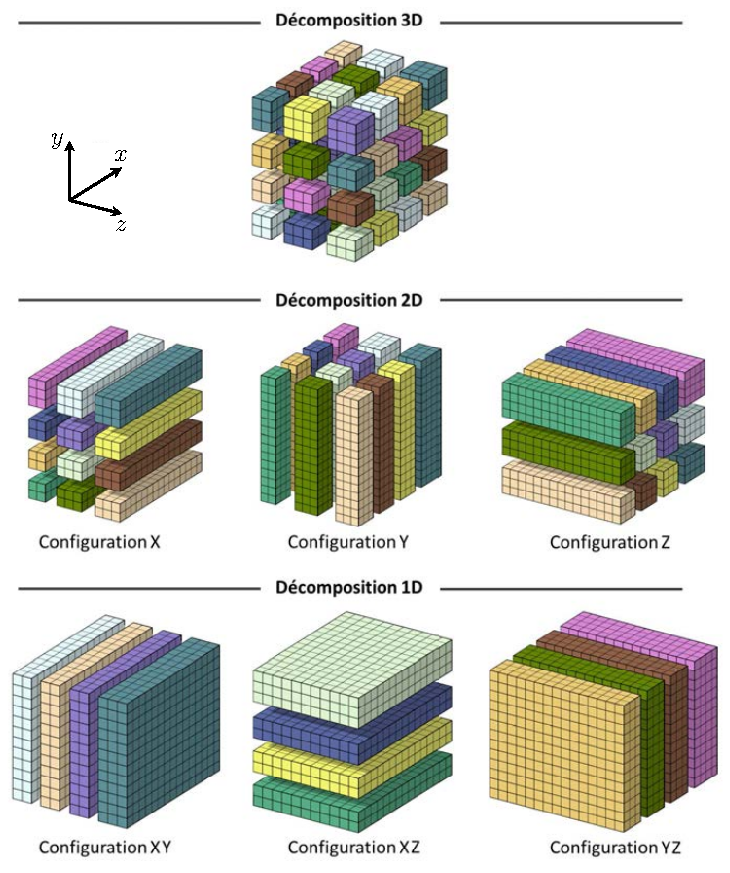
\includegraphics[width=0.8\linewidth]{Chap2/Pictures/Parallelisation/MULTIFAST_decompositions.pdf}
    \caption{Décomposition 1D, 2D ou 3D du domaine de calcul. Schéma tiré de la thèse de \cite{Bauer_PhDThesis}}
    \label{fig/MULTIFAST_decompositions}
\end{figure}

Il existe des nombres pour quantifier et qualifier la stratégie de parallélisation employée, à savoir l'accélération $Acc$ et l'efficacité $Eff$ (\cite{Tsoutsanis_Lecture}). L'accélération mesure le rapport des temps de calculs obtenus avec $n_{ref}$ (nombre de processeurs de référence) par rapport à $n_{procs}$, tel que $Acc(n_{procs}) = T(n_{ref}) / T(n_{procs})$. Sans tenir compte de la communication entre les cœurs, et en notant $\Delta T_{1}$ le temps nécessaire à la réalisation d'une itération, $T(n_{procs}) = n_{procs} \times \Delta T_{1}$. De même, $T(n_{ref}) = n_{ref} \times \Delta T_{1}$. Cela définit l'accélération idéale telle que $Acc_{id\acute{e}al} = n_{ref}/n_{procs}$. En réalité, le temps de communication a un grand impact sur le temps de calcul et devient prépondérant pour un très grand nombre de cœurs, ce qui fait chuter l'accélération. C'est pour cela que l'efficacité est généralement calculée. Elle est définie comme le produit entre l'accélération réelle et l'accélération idéale, $Eff(n_{procs})=Acc(n_{procs})/Acc_{id\acute{e}al}$. Plus le produit est proche de $1$, plus cela montre que la stratégie de parallélisation est efficace pour $n_{procs}$. Le code est alors extensible jusqu'à $n_{procs}$ cœurs en parallèle.\\

Les performances de parallélisation ont été mesurées sur la machine de calcul TURING du cluster de l'IDRIS lors de la thèse de \cite{Bauer_PhDThesis}. Chaque nœud de calcul de la machine était composé (lorsque les tests ont été effectués) de 16 cœurs de calcul possédant chacun 16 Go de RAM. La communication inter-nœuds était assurée par un réseau dont le débit était de 20 Go/s. Des tests simulant $1000$ itérations sur un maillage de $2048 \times 512 \times 512$ nœuds ont été effectuées sur un nombre de cœurs variant de $1024$ à $16384$. Les temps de calculs, les accélérations et les efficacités sont recensés dans le \cref{tab/perfo_MULTIFAST}. Les courbes d'accélération et d'efficacité sont disponibles en \cref{fig/perfo_MULTIFAST}. MULTIFAST est extensif jusqu'à $\approx 5000$ cœurs.

\begin{table}[!hbtp]
\centering
\begin{tabular}{|c||c|c|c|}
\hline
\textbf{$N_{procs}$} & \textbf{Temps par itération (s)} & \textbf{Accélération} & \textbf{Efficacité}\\ \hline
1024 & 2.789 & & \\
2048 & 1.389 & 2.000 & 1.004 \\
4096 & 0.706 & 3.950 & 0.988 \\
8192 & 0.380 & 7.339 & 0.917 \\
16384 & 0.242 & 11.525 & 0.720 \\ \hline
\end{tabular}
\caption{Performances parallèles du code. Tests effectués sur la machine de calcul TURING (cluster de l'IDRIS) un maillage contenant $2048 \times 512 \times 512$ nœuds. Les données sont tirées de la thèse de \cite{Bauer2015}.}
\label{tab/perfo_MULTIFAST}
\end{table}

\begin{figure}[!hbtp]
    \centering
    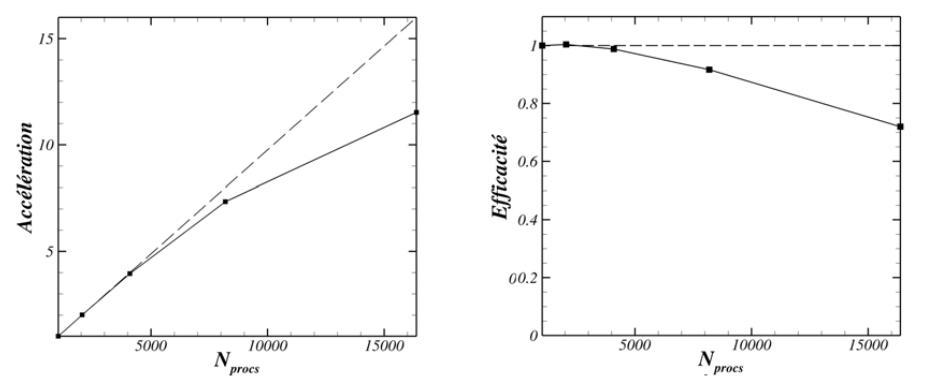
\includegraphics[width=\linewidth]{Chap2/Pictures/Parallelisation/perfo_MULTIFAST.png}
    \caption{Accélération (à gauche) et efficacité (à droite) de MULTIFAST. Tests effectués sur la machine de calcul TURING (cluster de l'IDRIS) sur un maillage contenant $2048 \times 512 \times 512$ nœuds. Les traits en pointillés correspondent au cas théorique. Les graphiques sont tirés de la thèse de \cite{Bauer2015}.}
    \label{fig/perfo_MULTIFAST}
\end{figure}

%%%%%%%%%%%%%%%%%%%%%%%%%%%%%%%%%%%%%%
\subsubsection{Domaine de calcul et arrangement des variables}
\label{subsubsec/domaine_calcul_arrangement_variables}

La \cref{fig/domaine_overview} montre le système de coordonnées utilisé dans MULTIFAST, ainsi que les vitesses et les conditions aux limites correspondantes. MULTIFAST simule des écoulements dans des boîtes rectangulaires de taille $L_{x} \times L_{y} \times L_{z}$ comme écrit plus haut. $x, y$ et $z$ (ou $u, v$ et $w$) désignent respectivement les directions (ou les vitesses) longitudinale, verticale et transversale. L'écoulement est considéré infini dans la direction transversale, d'où l'utilisation d'une condition de périodicité. Les parois sont matérialisées par une condition d'adhérence dans la direction verticale, i.e. avec une vitesse nulle sur la paroi ($u_{i}=0$). La condition utilisée est soit de type périodique, soit de type \foreignquote{french}{\textit{ouverte}} dans la direction longitudinale suivant les simulations.

\begin{figure}[!hbtp]
    \centering
    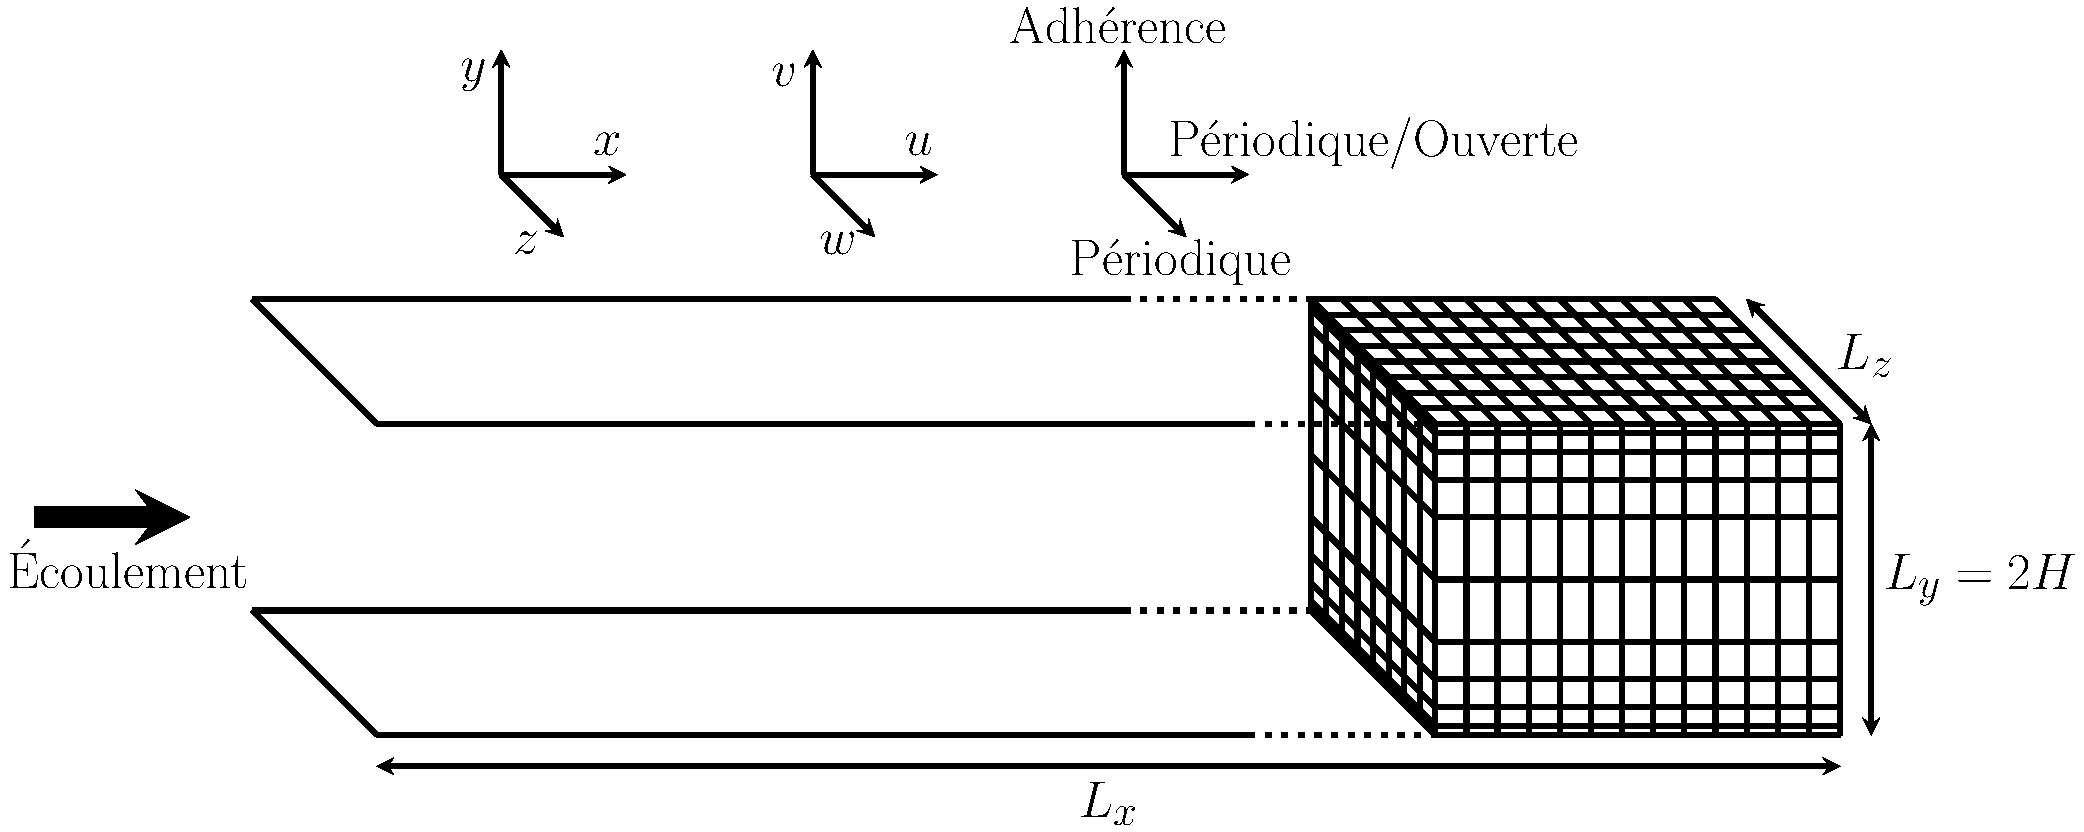
\includegraphics[width=\linewidth]{Chap2/Pictures/Domaine_calcul/Domaine_overview.pdf}
    \caption{Vue d'ensemble du domaine de calcul dans MULTIFAST et système de coordonnées associé.}
    \label{fig/domaine_overview}
\end{figure}

\vspace{2.5cm}
Un exemple de maillage généré par MULTIFAST est représenté sur la \cref{fig/domaine_overview}, à droite. Il est cartésien et est constitué de $n_{x} \times n_{y} \times n_{z}$ cellules. Les cellules sont distribuées uniformément dans les directions longitudinale et transversale. Une transformation tangentielle hyperbolique est utilisée permettant un raffinement près des parois dans la direction verticale. Deux types de transformations sont disponibles dans MULTIFAST. Elles seront présentées dans la sous-section.\\

\begin{figure}[!hbtp]
    \centering
    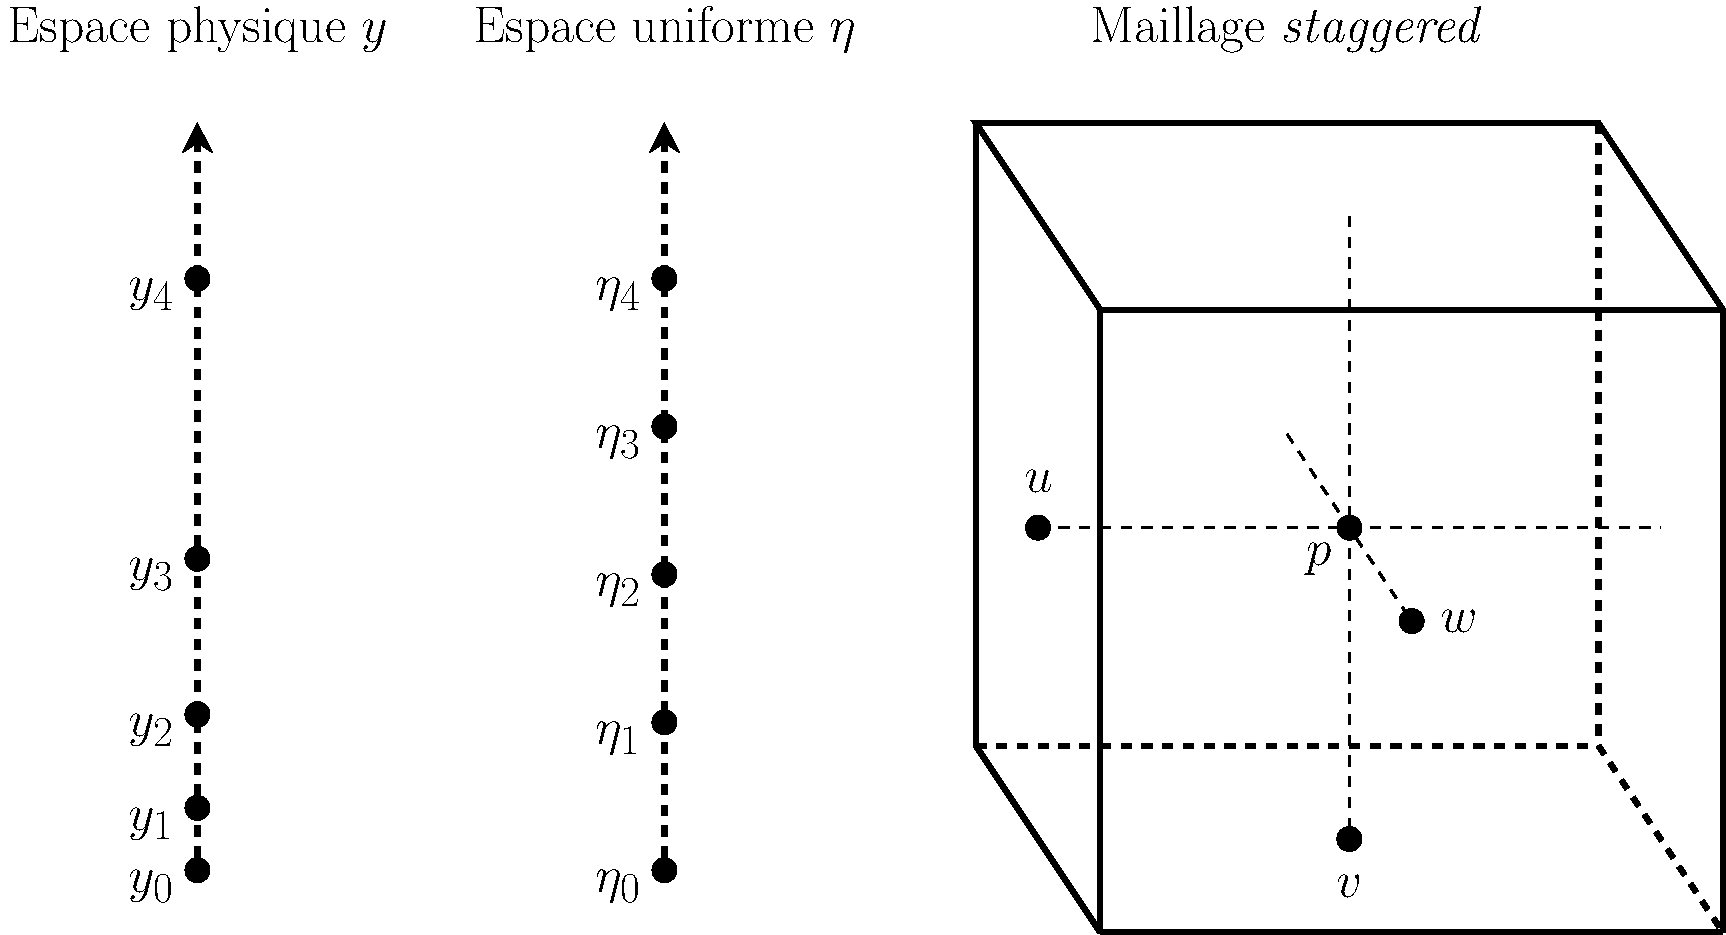
\includegraphics[width=0.75\linewidth]{Chap2/Pictures/Domaine_calcul/Node_MULTIFAST.pdf}
    \caption{Positions des vitesses et de la pression sur un nœud de maillage dans MULTIFAST et discrétisation de l'espace physique $y$ et de l'espace uniforme $n$.}
    \label{fig/node_MULTIFAST}
\end{figure}

La \cref{fig/node_MULTIFAST} montre l'arrangement des vitesses, $u,v$ et $w$, et de la pression $p$ sur un nœud de maillage dans MULTIFAST dans l'espace physique $y$ et l'espace uniforme $\eta$. Placer les vitesses, $u,v$ et $w$, et la pression à la même position dans la cellule provoque une amplification des modes les plus élevés du maillage ($kh \approx \pi)$ comme expliqué par \citet{Ferziger2002}. Cela génère donc des oscillations factices dans l'écoulement. Il est donc nécessaire d'utiliser une approche de type \foreignquote{french}{\textit{staggered}} pour éviter le problème. Les vitesses sont donc placées sur les centres des faces et la pression est placée au centre de la cellule.

%%%%%%%%%%%%%%%%%%%%%%%%%%%%%%%%%%%%%%%%%%%%%%%%%%%%%%%%%%%%%%%%%%%%%%%%%%%%%%%%%%%%%%%%%%%%%%%%%%%%%%%%%%%%%%%%%%%%%%%%%%%%%%%%%%%%%%%
\clearpage
\section{Conclusions}

\begin{itemize}

	% présentation générale du code
	\item Le code SND MULTIFAST est présenté en détail dans un premier temps. Il est basé sur une forme adimensionnelle des équations de Navier-Stokes et du transport de scalaire passif. Le fonctionnement du code, ainsi que les différents schémas numériques disponibles, sont explicités.

	% généralisation du code
	\item Les développements réalisés au cours de la thèse sont détaillés dans un second temps. Il a fallu implémenter la méthode Fringe afin de simuler les écoulements non-homogènes dans la direction longitudinale, tout en gardant les conditions aux limites périodiques. De plus, un module reposant sur la méthode des frontières immergées a été développé pour les simulations sur parois rugueuses.

	% validation et présentation des résultats théoriques importants
	\item Enfin, MULTIFAST est validé à travers un cas académique dans un troisième temps : un écoulement en canal turbulent développé à bas nombre de Reynolds avec transport d'un scalaire passif. Les résultats obtenus ont été post-traité grâce à l'outil PyFast (développé au cours de la thèse) et comparés à la littérature.


\end{itemize}
